\begin{figure}[t]
  \centering
  \begin{tikzpicture}
    \node[inner sep=0pt] (img1) at (0.0\textwidth, -0.0\textwidth)
         {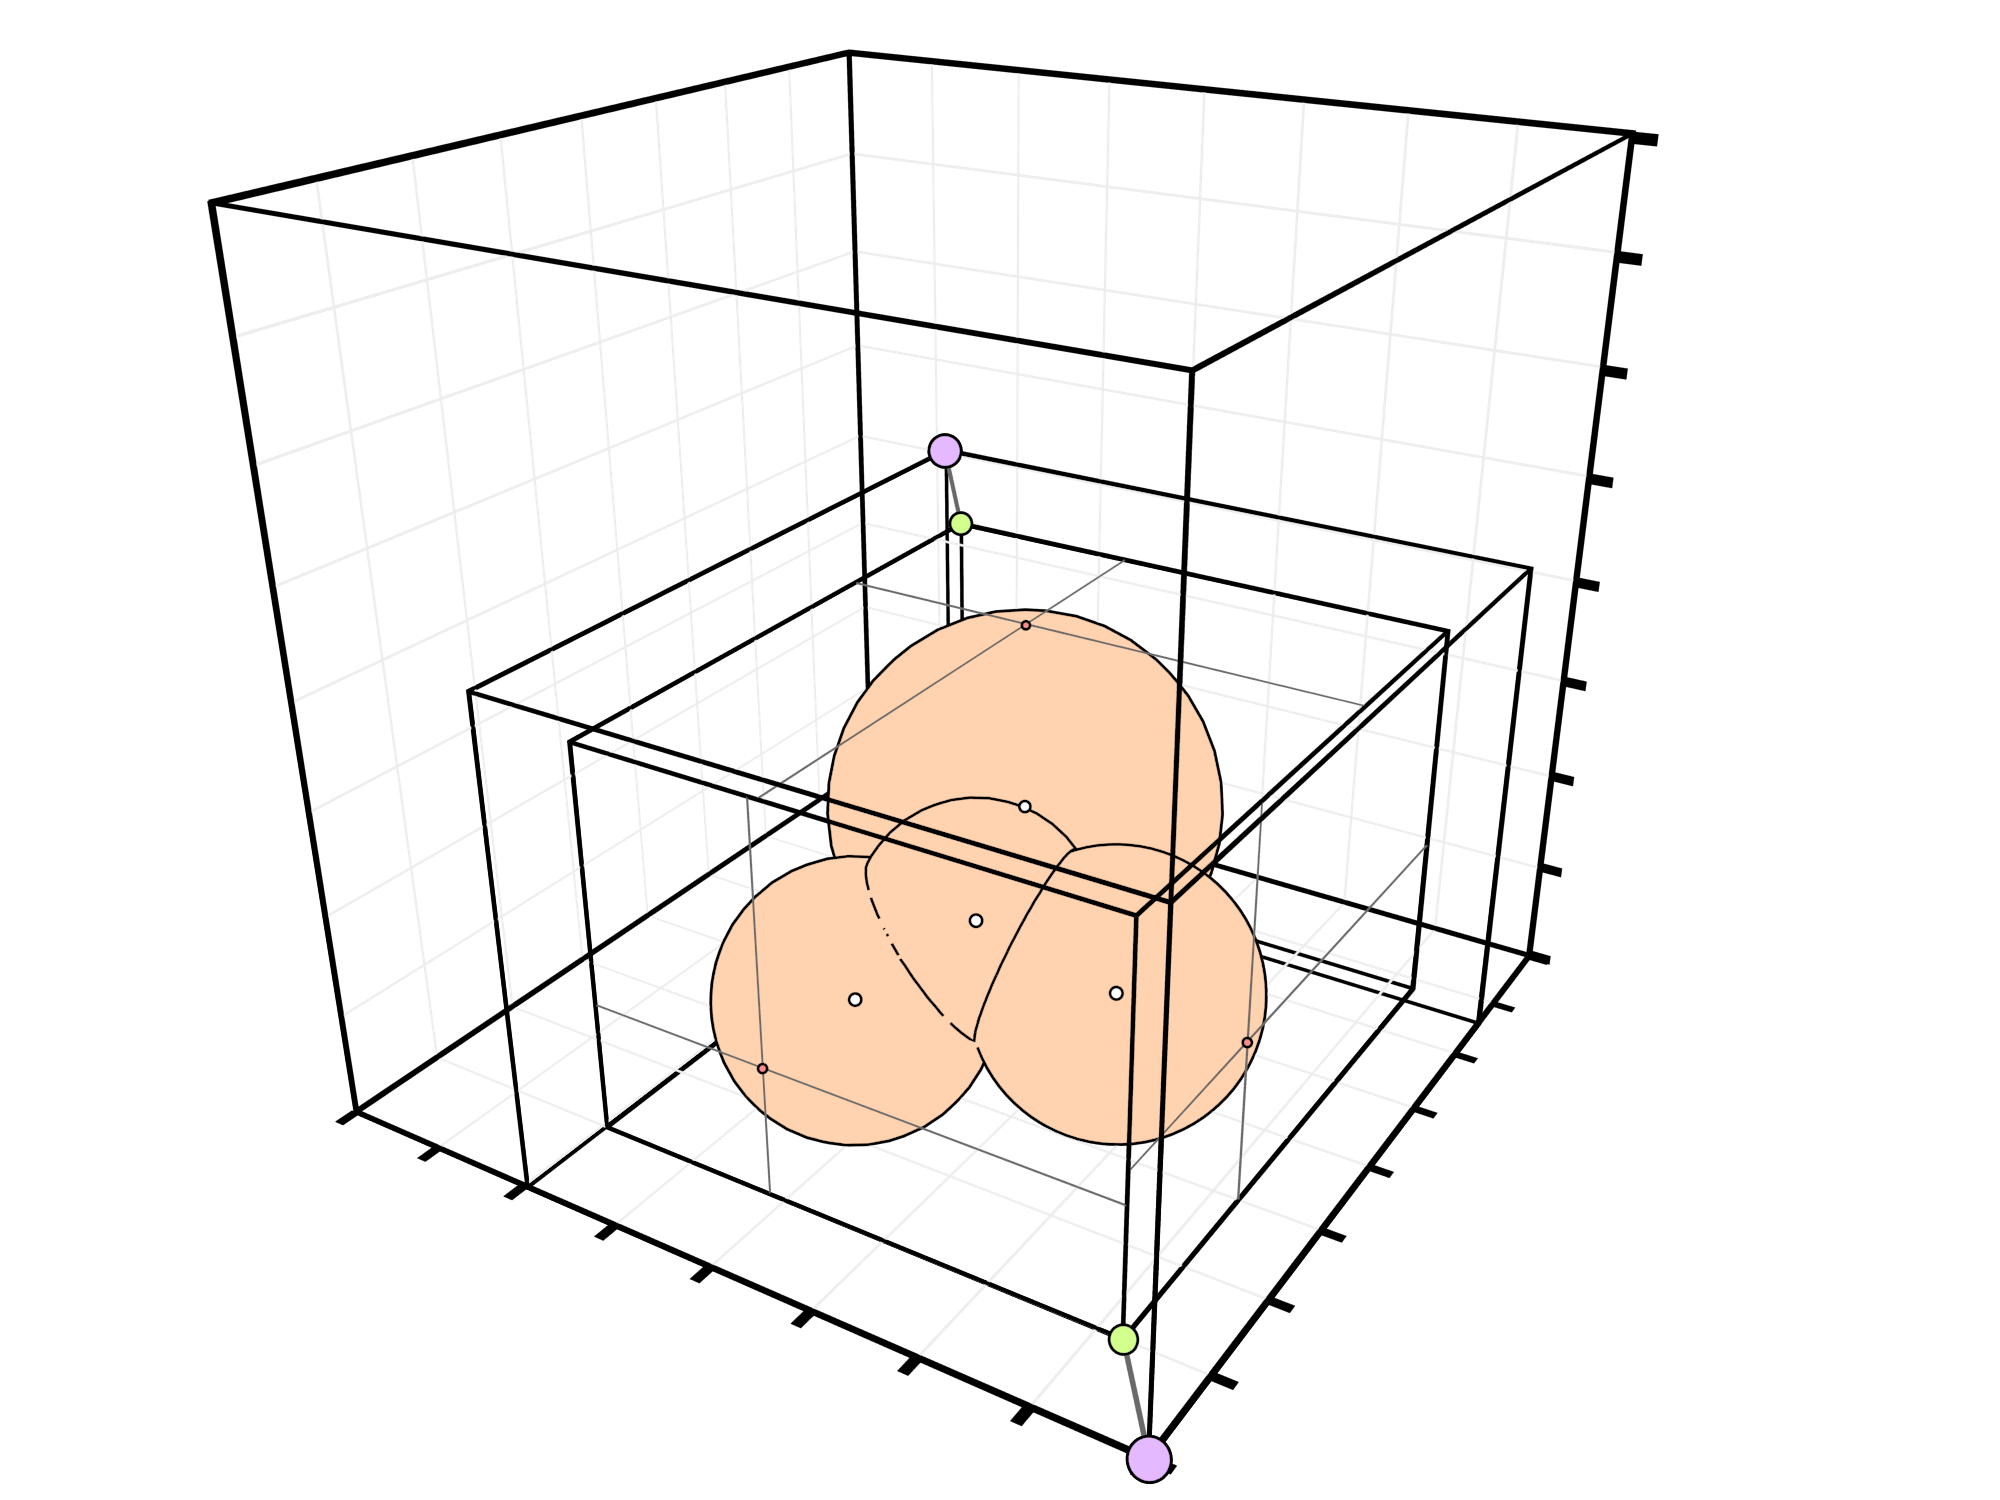
\includegraphics[width=12cm]{./img/raw/hs-opdeling-scene.png}};

    \node[] (camera-origin) at (0.225 * 16cm, -.08  * 16cm) {$2^l$};
    \node[] (camera-origin) at (0.075 * 16cm, -.28 * 16cm) {$\mathcal{O}$};
    \node[] (camera-origin) at (0.015  * 16cm, -.23  * 16cm) {$\mathbf{p}_\text{min}$};
    \node[] (camera-origin) at (0.015  * 16cm, .13  * 16cm) {$\mathbf{p}_\text{max}$};
  \end{tikzpicture}
  \caption{Een voorbeeld van de opdeling van de sc\`ene met behulp van een octree.}
  \label{fig:hs-opdeling-scene}
\end{figure}

